
% !TeX document-id = {a90a2b0a-e08e-44ed-850a-35793bedbf3a}
% !TeX TS-program = xelatex

% !BIB program = biber
\documentclass[handout]{beamer}
%\documentclass[compress]{beamer}
\usepackage[T1]{fontenc}
\usepackage{pifont}
\usetheme[block=fill,subsectionpage=progressbar,sectionpage=progressbar]{metropolis} 


\definecolor{Purple}{HTML}{911146}
\definecolor{Orange}{HTML}{CF4A30}

% Theme colors are derived from these two elements
\setbeamercolor{alerted text}{fg=Orange}

% ... however you can of course override styles of all elements
\setbeamercolor{frametitle}{bg=Purple}


\usepackage{wasysym}
\usepackage{etoolbox}
\usepackage[utf8]{inputenc}

\usepackage{threeparttable}
\usepackage{subcaption}

\usepackage{tikz-qtree}
\setbeamercovered{still covered={\opaqueness<1->{5}},again covered={\opaqueness<1->{100}}}


\usepackage{listings}

\lstset{
	basicstyle=\scriptsize\ttfamily,
	columns=flexible,
	breaklines=true,
	numbers=left,
	%stepsize=1,
	numberstyle=\tiny,
	backgroundcolor=\color[rgb]{0.85,0.90,1}
}



\lstnewenvironment{lstlistingoutput}{\lstset{basicstyle=\footnotesize\ttfamily,
		columns=flexible,
		breaklines=true,
		numbers=left,
		%stepsize=1,
		numberstyle=\tiny,
		backgroundcolor=\color[rgb]{.7,.7,.7}}}{}


\lstnewenvironment{lstlistingoutputtiny}{\lstset{basicstyle=\tiny\ttfamily,
		columns=flexible,
		breaklines=true,
		numbers=left,
		%stepsize=1,
		numberstyle=\tiny,
		backgroundcolor=\color[rgb]{.7,.7,.7}}}{}


\usepackage[american]{babel}
\usepackage{csquotes}
\usepackage[style=apa, backend = biber]{biblatex}
\DeclareLanguageMapping{american}{american-UoN}
\addbibresource{../literature.bib}
\renewcommand*{\bibfont}{\tiny}

\usepackage{tikz}
\usetikzlibrary{shapes,arrows,matrix}
\usepackage{multicol}

\usepackage{subcaption}

\usepackage{booktabs}
\usepackage{graphicx}

\graphicspath{{../pictures/}}

\makeatletter
\setbeamertemplate{headline}{%
	\begin{beamercolorbox}[colsep=1.5pt]{upper separation line head}
	\end{beamercolorbox}
	\begin{beamercolorbox}{section in head/foot}
		\vskip2pt\insertnavigation{\paperwidth}\vskip2pt
	\end{beamercolorbox}%
	\begin{beamercolorbox}[colsep=1.5pt]{lower separation line head}
	\end{beamercolorbox}
}
\makeatother



\setbeamercolor{section in head/foot}{fg=normal text.bg, bg=structure.fg}



\newcommand{\question}[1]{
	\begin{frame}[plain]
		\begin{columns}
			\column{.3\textwidth}
			\makebox[\columnwidth]{
				
\includegraphics[width=\columnwidth,height=\paperheight,keepaspectratio]{../pictures/mannetje.png}}
			\column{.7\textwidth}
			\large
			\textcolor{orange}{\textbf{\emph{#1}}}
		\end{columns}
\end{frame}}

\newcommand{\instruction}[1]{\emph{\textcolor{gray}{[#1]}}}


\title[Computational Communication Science 2]{\textbf{Computational Communication Science 2} \\Week 7 - Lecture\\ »Rule-based vs. Automated Text Classification«}
\author[Marthe Möller, Anne Kroon]{Marthe Möller \\ Anne Kroon \\ ~ \\ \footnotesize{a.m.moller@uva.nl, @marthemoller \\a.c.kroon@uva.nl, @annekroon} \\}
\date{May, 2022}
\institute[Digital Society Minor, University of Amsterdam]{Digital Society Minor, University of Amsterdam}


\begin{document}
	
	\begin{frame}{}
		\titlepage
	\end{frame}
	
	\begin{frame}{Today}
		\tableofcontents
	\end{frame}
	
	
	\section{Rule-based Text Classification}
	
	\begin{frame}{Text Classification} 
		
	Text classification: To assign a label to a text.
	
	For example, to distinguish between:
	\begin{itemize}
		\item newspaper articles about sports vs. economics.
		\item reliable vs. unreliable information about vaccination.
		\item webpages about holding companies vs. financing companies.
		\item positive vs. negative movie reviews.
	\end{itemize}
	
	\end{frame}
		
	\begin{frame}{Studying Flaming (Example)} 
	
	RQ: How problematic is flaming on Twitter? \\
	Bag-of-words approach:
	
	\begin{enumerate}
		\item Create a list with all the swearwords that exist.
		\item For each tweet in the dataset, use the list to count the number of swearwords	
	\end{enumerate}
	

\end{frame}


	\begin{frame}{Sentiment Analysis} 
	
	We can add nuance by creating more rules.
	
	For example, in sentiment analyses, we can include a rule telling the machine what to do in case of negation or modifiers.
	
	"This movie is really not good." \\
	"This movie is really good."
		
	\end{frame}


	\begin{frame}{Rule-based Text Classifcation} 
	
	Advantages of rule-based text classification:
	\begin{itemize}
		\item Simple and therefore transparent
		\item Cheap
	\end{itemize}
	
	Challenges of rule-based text classification:
	\begin{itemize}
		\item Not a suitable way to anayze latent or abstract variables 
		\item You must know all the categories beforehand
	\end{itemize}

	\end{frame}


\begin{frame}{From Rule-based to Automated}

	When it is easy for humans to decide to what class a text belongs, but we struggle to translate our decision process into straight-forward rules, we are likely to be better of using a form of automated text classification: Supervised Machine Learning.
	
\end{frame}


	
	\section{Automated Text Classification: SML}
	
	
	\begin{frame}{What is SML?}
		
		\begin{center}
			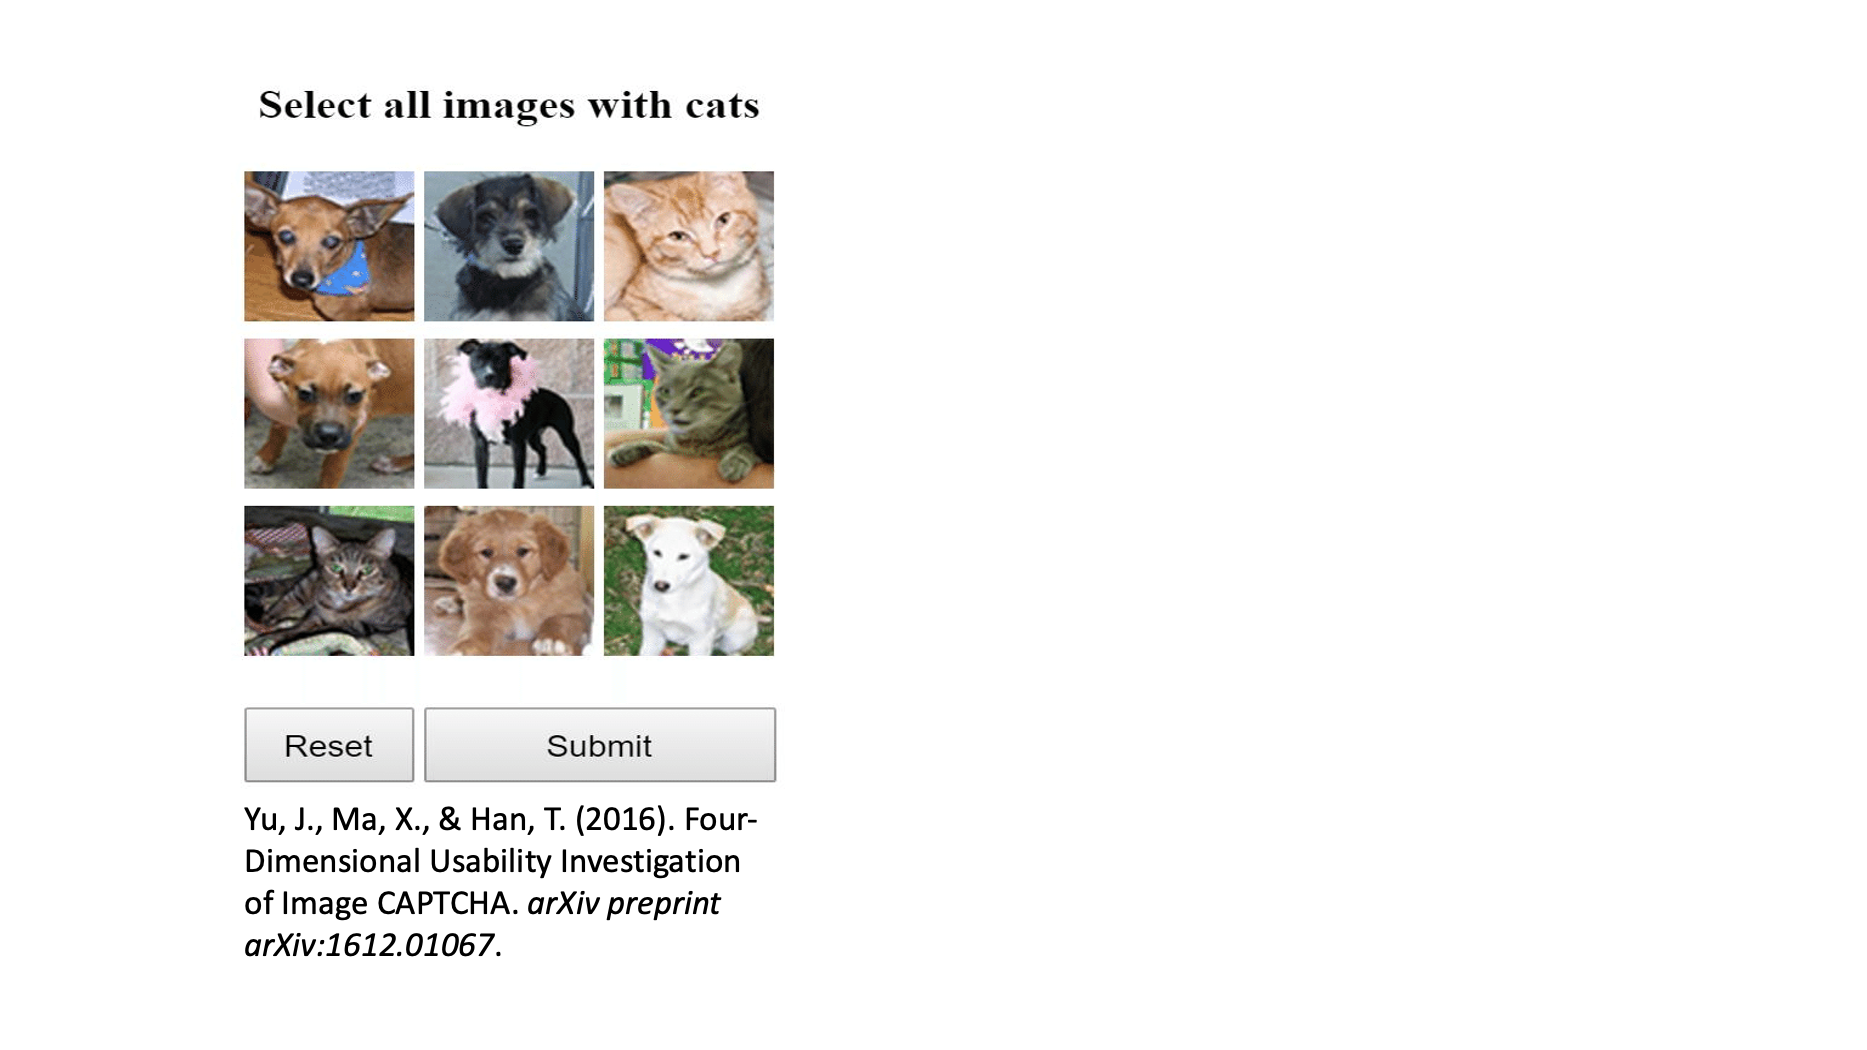
\includegraphics[width=4cm, height=7cm]{../pictures/CAPTCHA.png} 
		\end{center}
		
		
		% Probably all of you have come across an assignment like this one once when you tried to access a website. You asked to determine for each image if it depicts a cat. There are many variations to this assignment (e.g., select all the images with a traffic sign). The purpose of these assignments is to verify that a human is trying to enter a webpage as opposed to a machine. For this protection mechanism to work, it is assumed that while humans are able to distinguish pictures of cats from other pictures, machines cannot.
		
	\end{frame}
	
	
	\begin{frame}{What is SML?}
		
		\begin{center}
			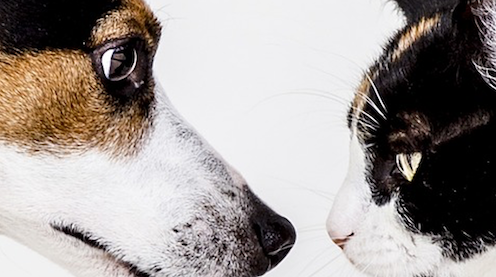
\includegraphics{../pictures/dogvscat.png}
		\end{center}
		
		\begin{tiny}
			Read more about this project in: 
			\fullcite{sermanet_overfeat_2014} 
		\end{tiny}
		
		
		% In 2013, Kaggle (Kaggle.com) challenged people to write a script teaching a computer to successfully complete the task of distinguishing images of cats from images of dogs.
		
		% To achieve their goal, contesters needed to use Machine Learning.
		
	\end{frame}
	
	\begin{frame}{What is SML?} 
		
		Machine Learning: A process whereby a machine learns how to predict a variable.
		
		% In this story, it is the process whereby the computer learns how to predict images’ score on a variable (let’s name it ‘animal’) which can be either (1) cat or (0) dog.
		
	\end{frame}
	
	
	\begin{frame}{What is SML?} 
		
		Supervised Machine Learning (SML): “A form of machine learning, where we aim to predict a variable that, for a least part of our data is known.” \\\
		
		“The goal of Supervised Machine Learning: estimate a model based on some data, and then use the model to predict the expected outcome for some new cases, for which we do not know the outcome yet.” \\\
		
		\begin{tiny}
			\fullcite{van_atteveldt_computational_2022} 
		\end{tiny}
		
		
		
		% In this lecture, we focus on a specific type of machine learning, namely supervised machine learning.
		
		% In the cats-example, it would work as follows: We give the computer part of the images in a dataset, along with their scores on the animal-variable. Based on this part of the dataset, the computer “learns” which factors determine whether an image receives score 1 (cat) or score 0 (dog). The computer applies this to the remaining images (for which it was unknown whether they depicted a dog or a cat). So, the computer has ‘learned’ to distinguish cats from dogs. 
		
	\end{frame}
	
	\begin{frame}{What is SML?} 
		
		Machine Learning has a lot of similarities to regression analysis!
		
		% Communication scholars often use scores on some independent variables (for example: age, and gender) to calculate subjects’ scores on a dependent variable (for example: Instagram usage). They use a regression analysis to do this calculation.
		
	\end{frame}
	
	
	\section{The principles behind SML}
	
	\begin{frame}{The principles behind SML} 
		
		\(y = constant + b_1 * x_1 + b_2 * x_2\) 
		
		\(x_1\) = bark? (0= no, 1 = yes) \\\
		\(x_2\) = tail? (0 = no, 1 = yes) \\\
		\(y\) = Is this a dog? ( 0 = definitely no, 1 = definitely yes)
		
		% [Discuss the meaning of the formula, the constant and the regression coefficient]. By running the regression analysis, we retrieve values for the regression coefficients and the constant.
		
	\end{frame}
	
	
	\begin{frame}{The principles behind SML} 
		
		\(y = constant + b_1 * x_1 + b_2 * x_2\) \\\
		
		\(y = 0 + 0.8 * x_1 + 0.2 * x_2\) \\\
		
		\(y = 0 + 0.8 * 1 + 0.2 * 0\) \\\
		
		% If we then fill out the scores of a participant on each independent variable, we can predict that person’s score on the dependent variable.
		
	\end{frame}
	
	\begin{frame}{The principles behind SML} 
		
		\(y = 0 + 08 * 1 + 0.2 * 0\) \\\
		
		\(0.8 = 0 + 0.8 * 1 + 0.2 * 0\) \\\
		
		% A computer could do this for an unlimited number of participants. So, say we have 1000 people. With the regression formula, we can predict for each person if they have an Instagram account or not based on their gender and age.
		
	\end{frame}
	
	\begin{frame}{The principles behind SML} 
		
		\(0.8 = 0 + 0.8 * 1 + 0.2 * 0\) \\\
		
		Classification: a predictive modeling problem where a class label is predicted for a given example of input data. 
		
		
		%(https://machinelearningmastery.com/types-of-classification-in-machine-learning/)
		
		% Note that while in more traditional research approaches, we focus on the value of the regression coefficient (e.g., the coefficient for education level or what is the effect of education on Instagram usage), in machine learning, we do not care so much about the exact regression coefficients. We merely use the coefficients to predict. 
		
		%These predicting tasks are known as classification. 
		
		
	\end{frame}
	
	
	\begin{frame}{The principles behind SML}
		
		\begin{center}
			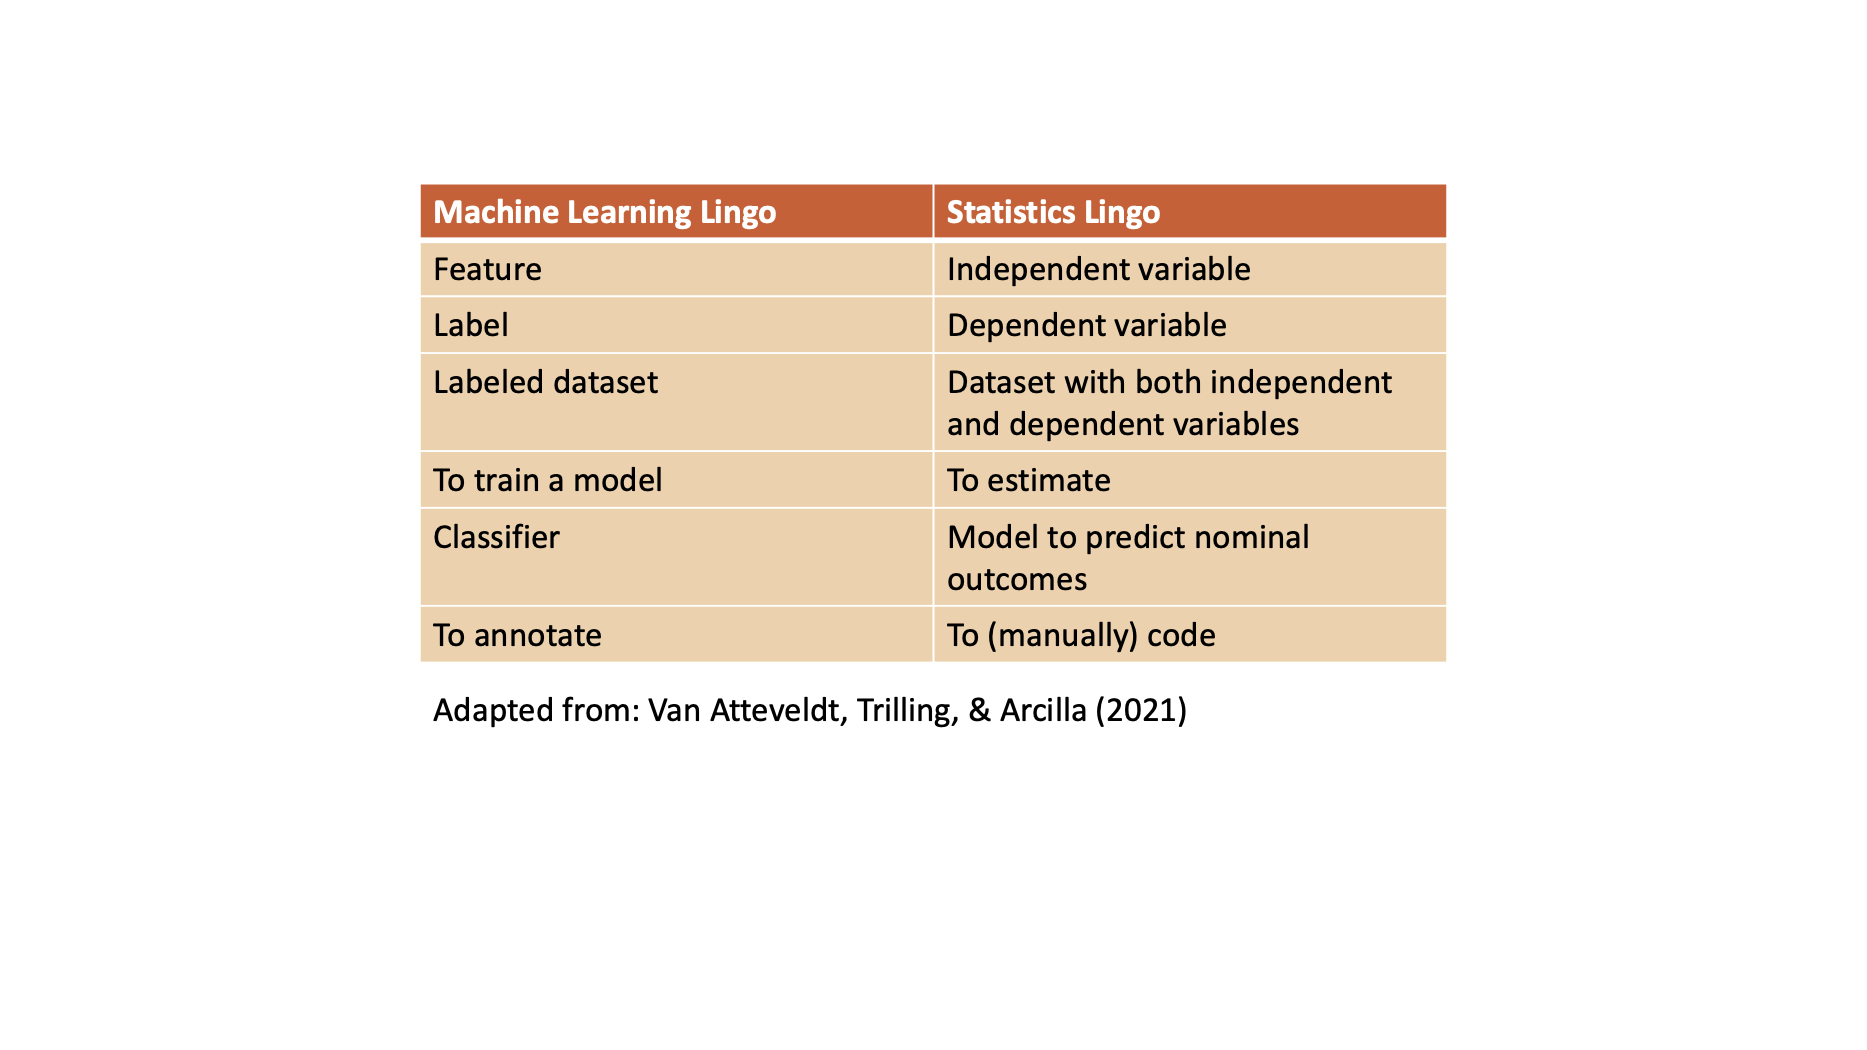
\includegraphics[width=\linewidth,height=\textheight,keepaspectratio]{../pictures/MLlingo.png} \\\
		\end{center}
		
		
		% Now that we are drawing comparisons between statistics and machine learning, let’s have a look at some machine learning lingo that you’ll bound to bump into.
		
	\end{frame}
	
	
	\begin{frame}{The principles behind SML} 
		
		Machine Learning: using a (regression) formula to predict a label. \\\
		
		Traditional usage of formulas in CS: to explain \\\
		
		Usage of formulas in ML: to predict \\\
		
		
		% ML is basically using something you already know to achieve a new goal.
		
		
	\end{frame}
	
	
	
	\begin{frame}{Zooming out} 
		
		We talked about:
		\begin{itemize}
			\item The principles behind SML \\\
		\end{itemize}
		
		Next, we will talk about:
		\begin{itemize}
			\item The steps of SML
		\end{itemize}
		
	\end{frame}
	
	
	\section{SML step by step}
	
	\begin{frame}{SML step by step}
		
		\begin{center}
			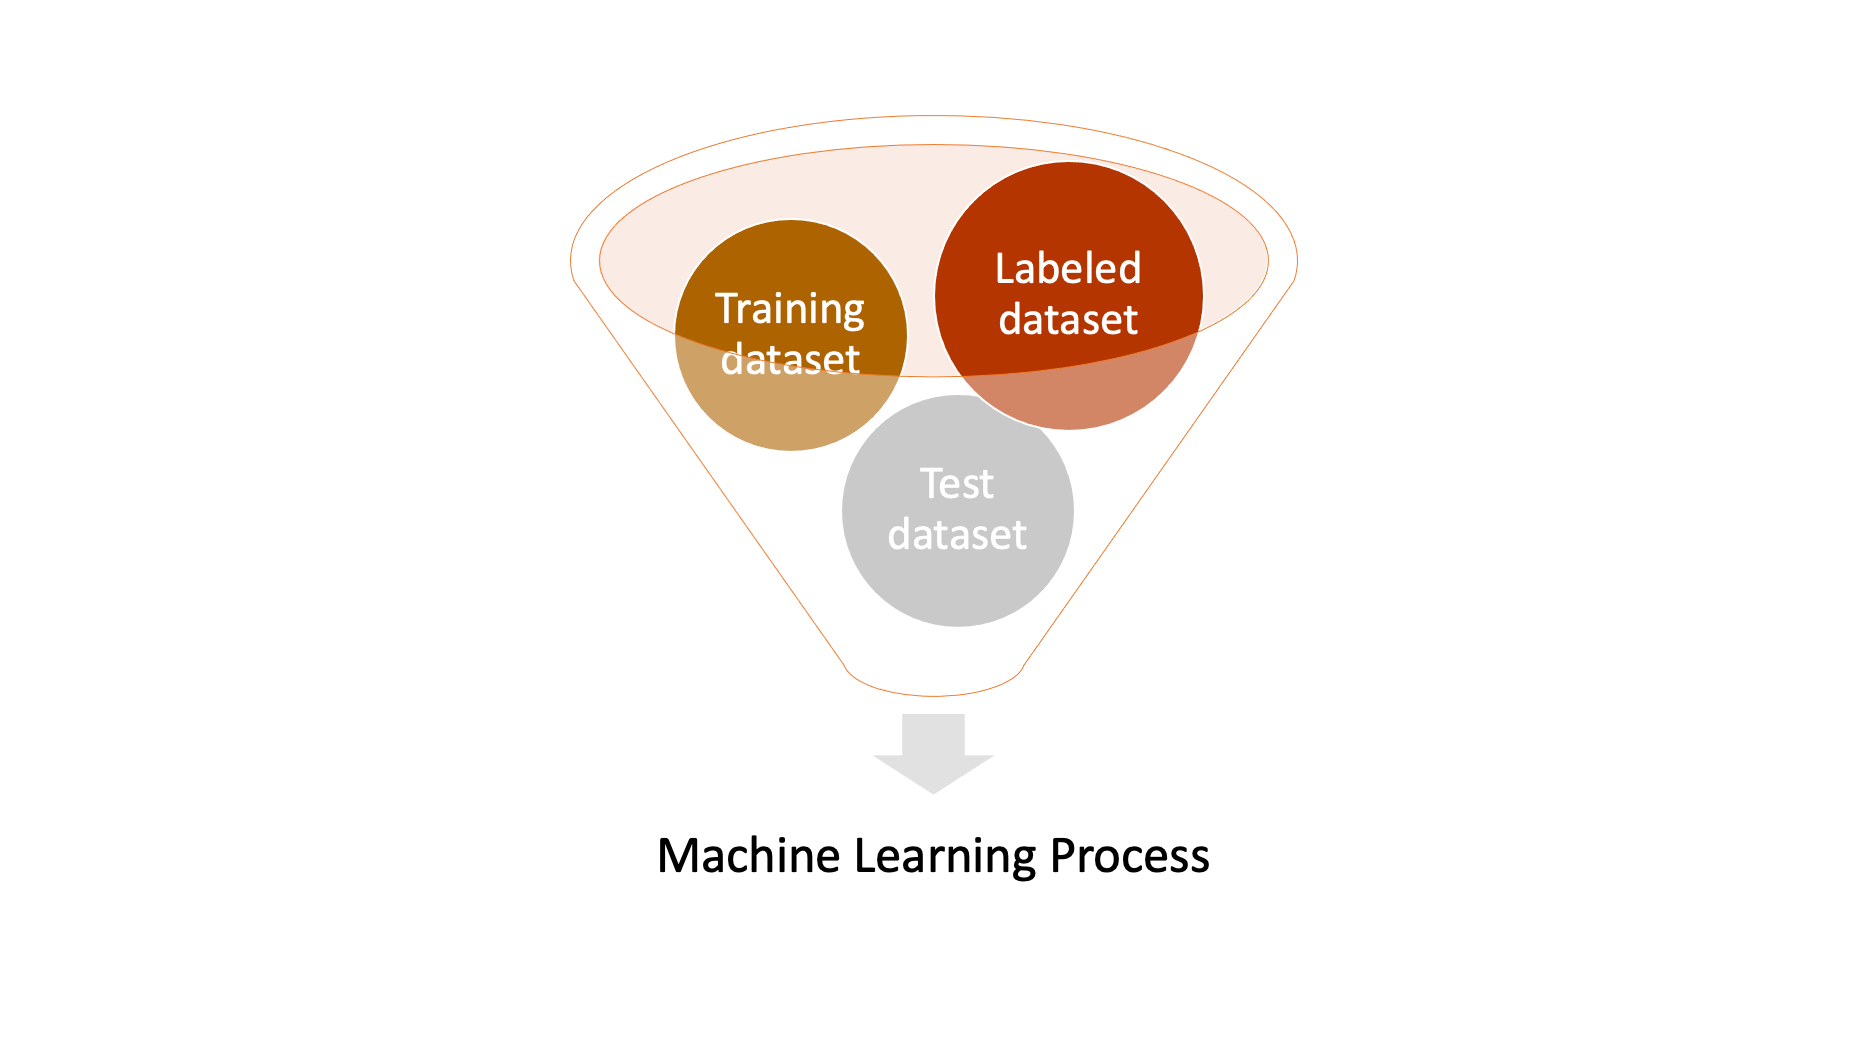
\includegraphics[width=\linewidth,height=\textheight,keepaspectratio]{../pictures/MLingredients.png} \\\
		\end{center}
		
		
		% To do SML, we need some ingredients. Namely, we need a labelled dataset. This is a dataset where for each case, the vales of the features (independent variables) and the labels (dependent variables) are known. We split this dataset into two parts. One part we call the training dataset and the other part we call the test dataset.
		
	\end{frame}
	
	
	\begin{frame}{SML step by step}
		
		\begin{center}
			
\includegraphics[width=\linewidth,height=\textheight,keepaspectratio]{../pictures/MLprocess.png} \\\
		\end{center}
		
		
		% With these ingredients, we can go through three steps.
		
		% First, we train our classifier, that is to say: We estimate our model using the training dataset.
		
		% If we connect this back to the regression equation we discussed earlier: We estimate the regression equation.
		
		% Second, we test our classifier: We test how capable our model is to predict the correct labels. We do this using the test dataset.
		
		% (Why not use the same training dataset again? We could do this, but it would be a rather lenient test because the classifier has been trained on exactly these data. To truly assess how well our classifier performs, we need to use new data. We use the test data because for these data, we can verify if the classifier was correct (remember that the test data stems from our labeled dataset, so we know what the correct labels are!).
		
		% Third, we evaluate our classifier:
		% More about this later today and this week!
		
	\end{frame}
	
	
	
	\begin{frame}{SML step by step}
		
		\begin{center}
			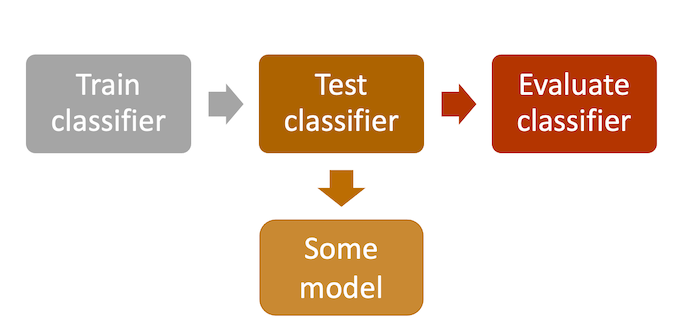
\includegraphics[width=\linewidth,height=\textheight,keepaspectratio]{../pictures/MLprocess_model.png} \\\
			
			Next class, we look at some commonly used ML models and at the process of evaluating classifiers.
		\end{center}
		

		
		% [connect each step to Van Zoonen & Van der Meer for an example]
		% [note here the important assumption of SML: that the training set, test set, and the unlabeled data that are to be classified are (at least in principle and approximately) drawn from the same population. For example, you cannot train a classifier using movie reviews and then use that classifier to analyze Instagram comments]
		
		
	\end{frame}
	
	
	\begin{frame}{Zooming out} 
		
		Today, we talked about:
		\begin{itemize}
			\item The principles behind SML
			\item The steps of SML \\\
		\end{itemize}
		
		Next, we will talk about:
		\begin{itemize}
			\item Some commonly used ML models
			\item Validating models
			\item The strengths and challenges associated to ML
		\end{itemize}
		
	\end{frame}
	
	
\end{document}